\chapter{Robotvezérlés környezete}
\section{Robotirányítás}
Robotirányításhoz szükséges, hogy legyen egy mechanikai rendszer, ez a robot azon részrendszere, amely az akciót valósítja meg. Az akció során szükség lehet a robot mozgatására a környezetben,
ezt a helyváltoztató berendezés végzi. Motorok, különböző mechanikai tagok teszik lehetővé a helyváltoztatást. A szenzoros rendszer belső állapota maga a mechanikai rendszer állapota, míg a külső állapot a környezet állapotát jellemzi.
Sokféle külső környezeti állapot létezik. Ahhoz, hogy a különböző környezeti tényezőket, például hőmérséklet, fényerősség, mágnesesség, láthatóvá és érzékelhetővé tegyük a robotunk számára, fel kell szerelni a megfelelő szenzorokkal.  \cite{robtel}
A dolgozat során egy Mantis Q drónt (\ref{fig:mantisq}. ábra) használunk robotként, a többit szimuláljuk.

\begin{figure}
	\centering
	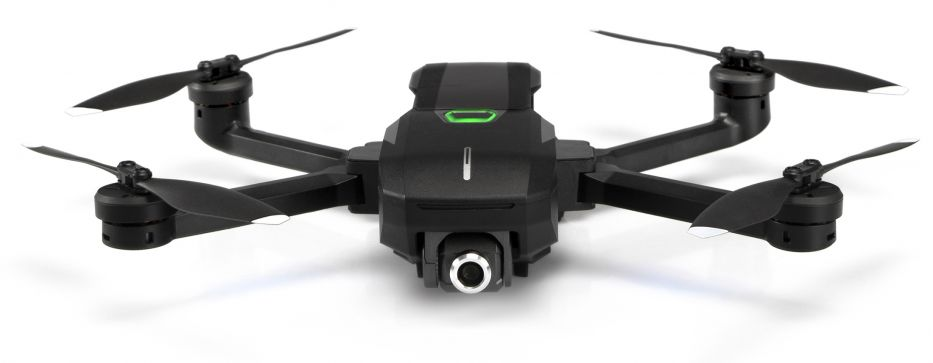
\includegraphics[width=\linewidth]{figures/mantisq.jpg}
	\caption{Yuneec Mantis Q \cite{mantisq}}
	\label{fig:mantisq}
\end{figure}

\section{Robot operációs rendszer - ROS}
Bármilyen robot rendelkezik különféle eszközökkel amivel érzékelik a világot és mozognak benne. A Robot operációs rendszer egy nyílt forráskódú könyvtárakat és eszközöket kínál a szoftverfejlesztés segítségére robotot, mint hardvert irányító alkalmazások létrehozásához. Hardver abszrakciót, driver-eket, könyvtárakat, megjelenítőket, üzenetek továbbítását, csomagkezelést és más szolgáltatást is nyújt. \cite{roswiki}
A ROS node-ok kommunikálni tudnak egymással, a szolgáltatások, hogy kérést küldjenek és választ kapjanak a node-ok között. A \emph{rosservice} szolgáltatással kapcsolódhatunk a ROS szerveréhez.
A \emph{roslaunch} utasítás egy .launch kiterjesztésű fájl alapján indít egy robotot, a megadott paraméterekkel.
\section{Kommunikáció - Mavros, Mavlink}
A MAVLink egy egyszerű üzenetküldési protokoll a drónokkal (és a fedélzeti drónkomponensek között) történő kommunikációhoz.A MAVLink hibrid publish-subscribe és point-to-point tervezési mintát követi. Az adatfolyamok témákként kerülnek elküldésre / közzétételre, míg a konfigurációs alprotokollok, például a missziók vagy a paraméterek point-to-point közötti újraküldéssel. Az üzeneteket az XML fájlok határozzák meg. Minden XML fájl meghatározza az adott MAVLink rendszer által támogatott üzenetkészletet. \cite{mavlink} A MAVLink nagyon hatékony, extrém kicsi az overhead, így QoS célra ideális. \\
\noindent
A mavros egy ROS kiegészítő, amely megvalósítja a MAVLink kommunikációját a ROS-t futtató számítógépek, a MAVLink-kompatibilis autopilotok és a MAVLink-kompatibilis Ground Control Station (GCS) között.
\section{Vezérlő - PX4}
\section{Szimulációs környezet - Gazebo}
\section{Együttes működés}